\chapter{Introduction} \label{chap:intro}
This is a citation \autocite{juliani2018unity}!
\begin{figure}
    \centering
    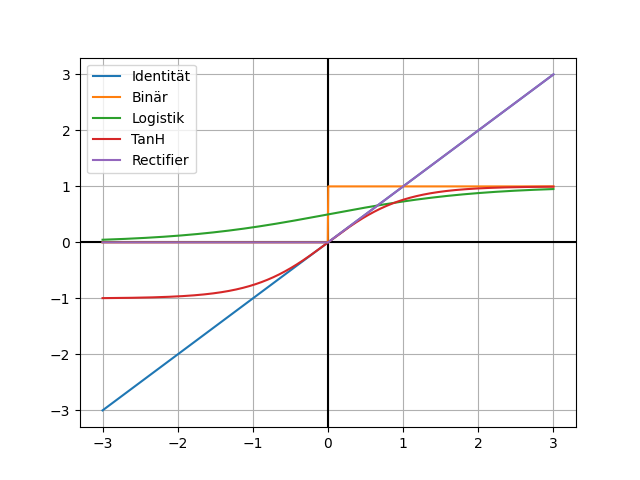
\includegraphics[width=0.8\textwidth]{img/test.png}
    \caption{Einige typische Aktivierungsfunktionen}
    \label{fig:actfn}
\end{figure}

\begin{figure}
    \centering
    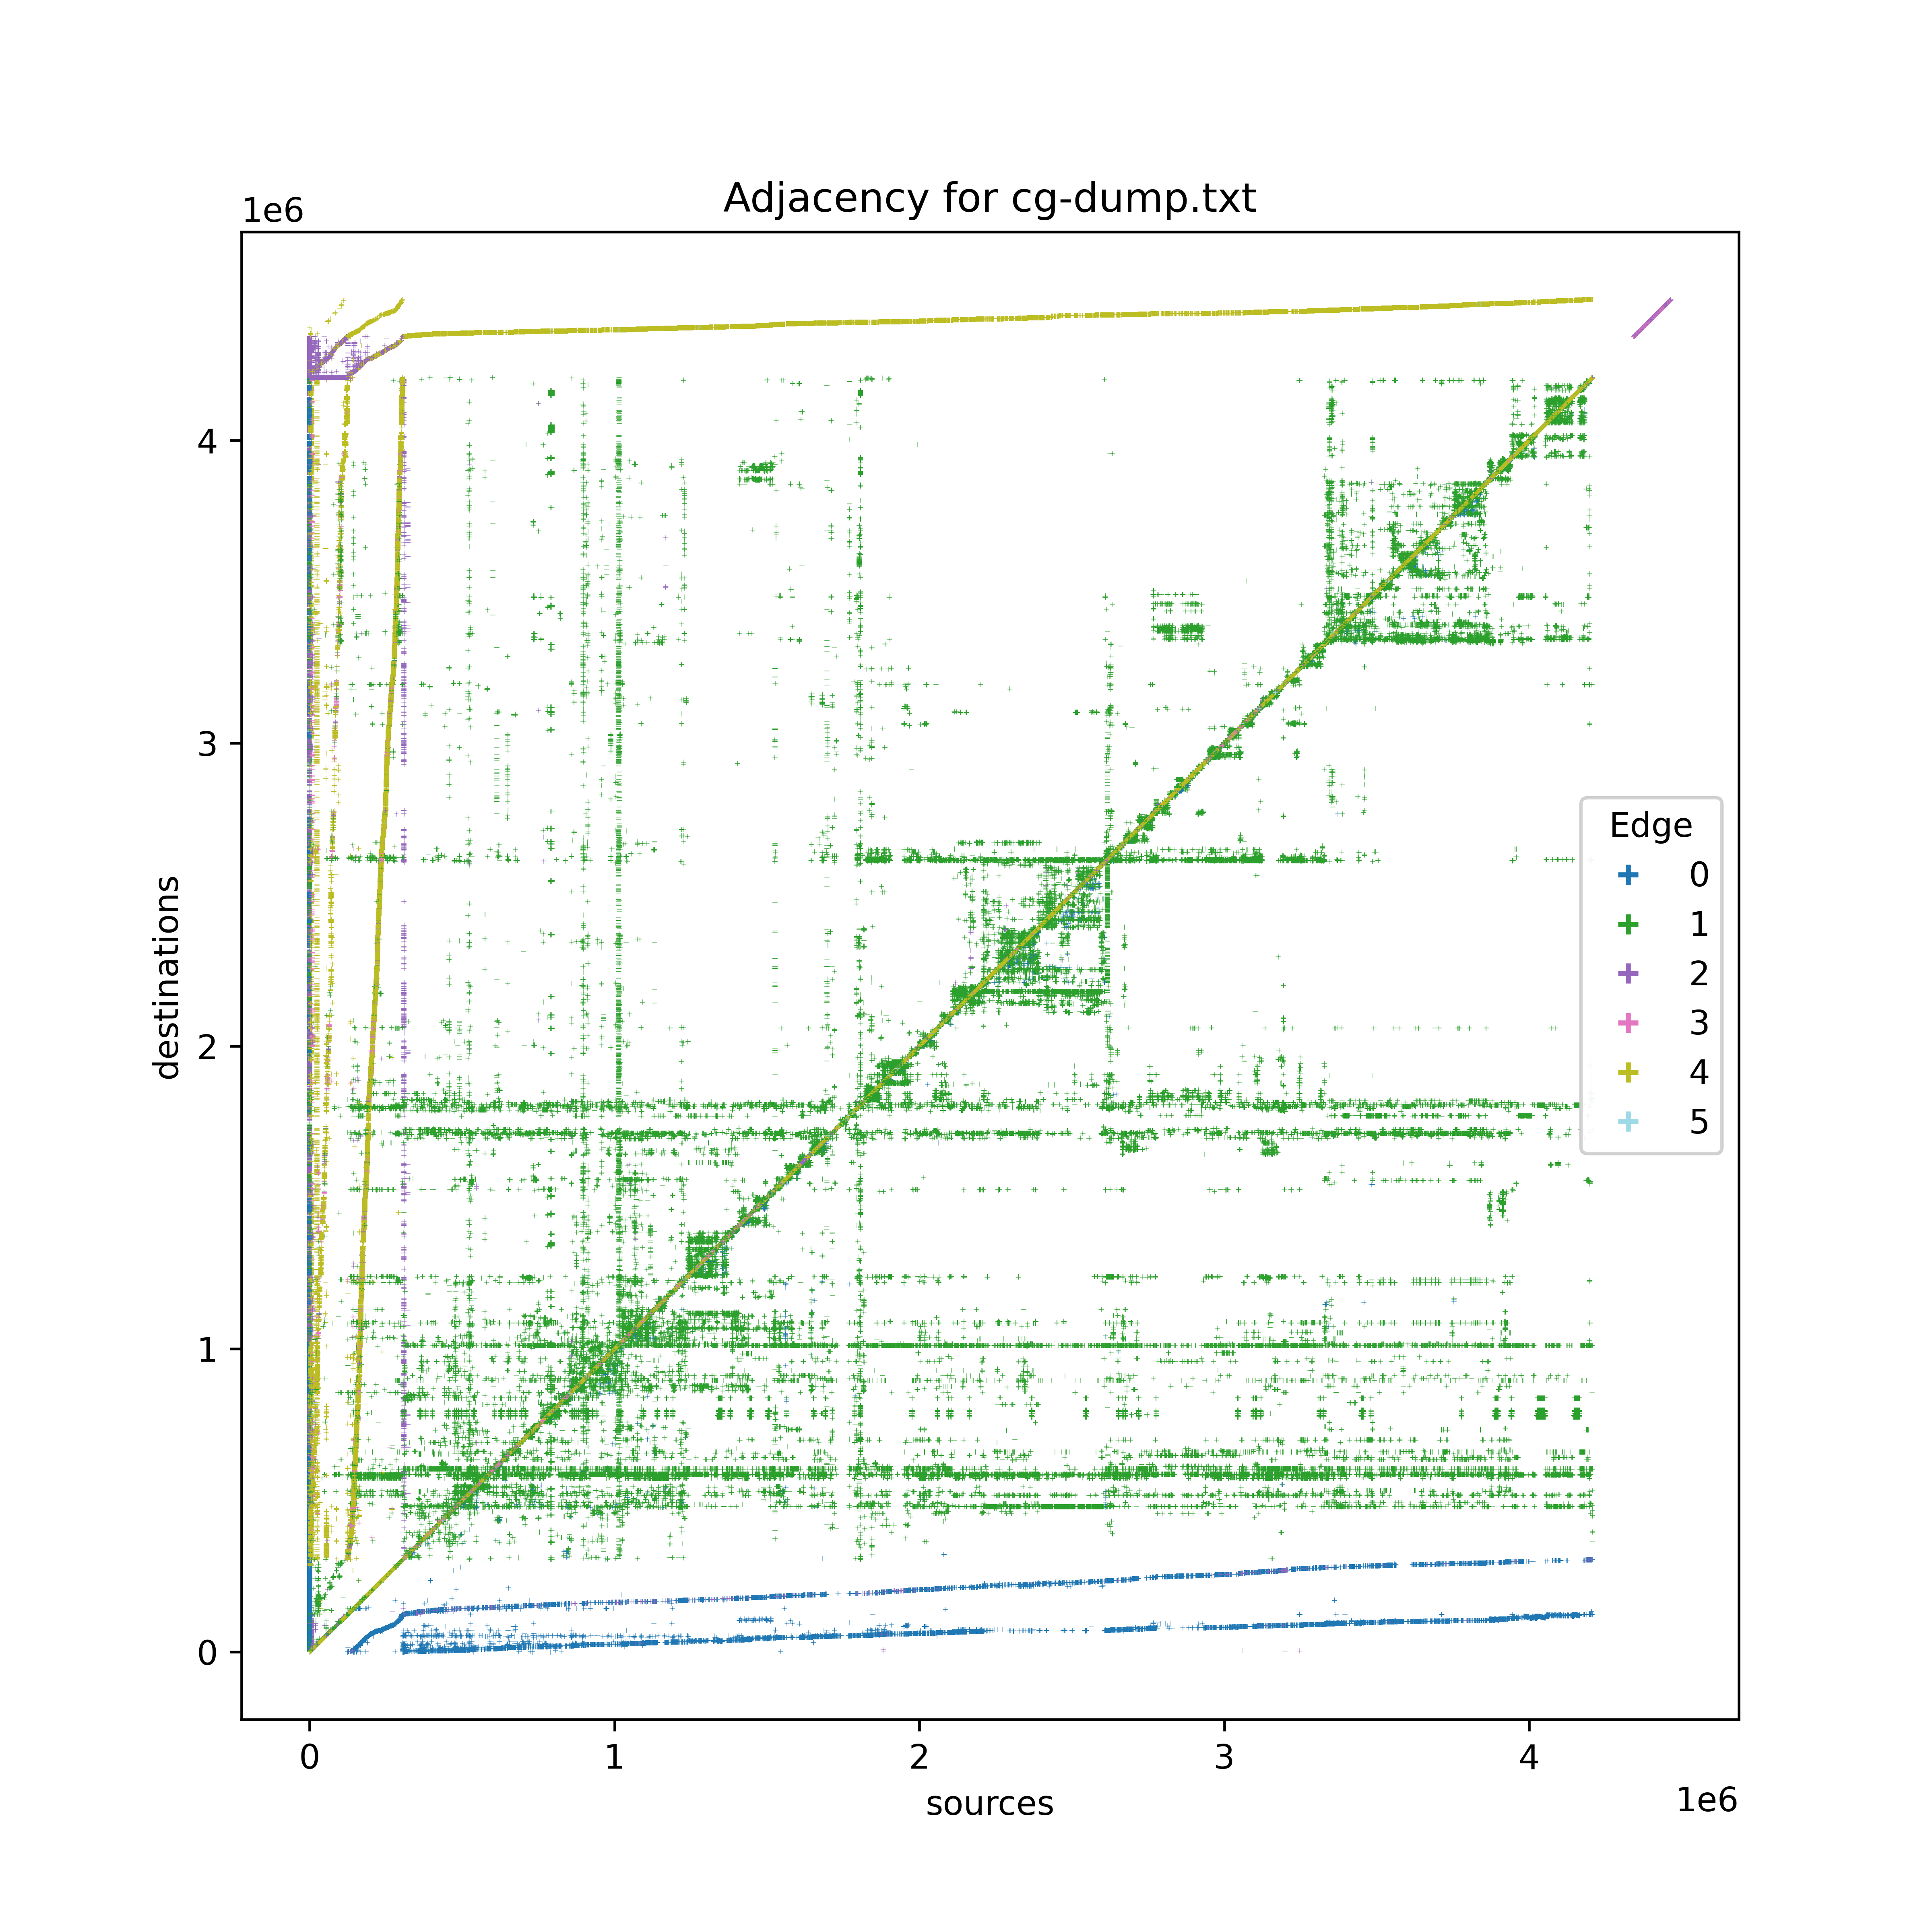
\includegraphics[width=1.\textwidth]{img/linux-consg.png}
    \caption{Adjacency Plot for the Constraint Graph of the Linux Kernel}
    \label{fig:linux-consg}
\end{figure}

\begin{minted}[mathescape, linenos]{python}

    # Note: $\pi=\lim_{n\to\infty}\frac{P_n}{d}$
    title = "Hello World"

    sum = 0
    for i in range(10):
     sum += i
\end{minted}



\begin{table}[h!]
    \begin{center}
        \caption{More rows.}
        \label{tab:table1}
        \begin{tabular}{l|S|r}
            \textbf{Value 1} & \textbf{Value 2} & \textbf{Value 3} \\
            $\alpha$         & $\beta$          & $\gamma$         \\
            \hline
            1                & 1110.1           & a                \\
            2                & 10.1             & b                \\
            3                & 23.113231        & c                \\
            4                & 25.113231        & d                \\ % <-- added row here
        \end{tabular}
    \end{center}
\end{table}


\section{Structure of this Thesis}

\section{Pointer Analysis}
what is pta; survey \autocite{hind2001pointer} and \autocite{toman2017taming} and \autocite{smaragdakis2015pointer}; theoretical complexity of parallel andersen analysis \autocite{mathiasen2021fine}

\subsubsection{Notions of Sensitivity}
field - flow - context - array sensitivity; structure sensitivity: \autocite{balatsouras2016structure}
\subsubsection{Steengards Analysis}
general idea
\subsubsection{Andersens Analysis}
inclusion based pta idea, timeframe
\subsubsection{Wave Propagation}
explain optimizations in modern sequential pta implementations: diffpts, worklists, consed hashes, \autocite{pereirawave}
\section{LLVM}
what is llvm, general compiler architecture: front / backends, llvm-IR
\subsection{Overview of Instructions}
go through instrs, and how they are relevant to pta, explain constraints \autocite{lin2015alias}
\section{Related Work}
\subsection{Context Free Languages}
first general idea: \autocite{reps1998program} first idea of gemm for cflpq \autocite{azimov2018context} kronecker product idea \autocite{orachev2020context} evaluation \autocite{mishin2019evaluation} spbla library \autocite{orachev2021spbla}, current draft [Taming Transitive Redundancy for Context-Free Language Reachability] fron SVF, parallel pta via cfl \autocite{su2014parallel}
\subsection{Sequential Analyses}
\subsubsection{SVF}
svf idea, built on top of llvm, \autocite{sui2016svf}, briefly explain all subcomponents i.e. memleak detection: \autocite{sui2014detecting} demand driven VF: \autocite{sui2018value} new alternative, faster, better results than svf \autocite{shi2018pinpoint}
\subsection{GPU Accelerated Analyses}
\subsubsection{Graspan}
original idea \autocite{zheng2008demand} big data approach on cpu \autocite{wang2017graspan} and gpu \autocite{zuo2021systemizing} alternative impl \autocite{gu2020towards} based on \autocite{mendez2012gpu} and \autocite{mendez2010parallel}
\section{Motivation}
general alias analysis is undecidable
\subsection{Static Analysis in Software Development}
finding bugs is becoming harder

inter procedural analysis scalability; create a single machine implementation that used parallel hardware and integrates into SVF
